% Chapter 5

\chapter{Extracción de características del iris en condiciones no ideales} % Main chapter title

\label{Capítulo 5} % For referencing the chapter elsewhere, use \ref{Chapter5} 

%----------------------------------------------------------------------------------------

% Define some commands to keep the formatting separated from the content 
%\newcommand{\keyword}[1]{\textbf{#1}}
%\newcommand{\tabhead}[1]{\textbf{#1}}
%\newcommand{\code}[1]{\texttt{#1}}
%\newcommand{\file}[1]{\texttt{\bfseries#1}}
%\newcommand{\option}[1]{\texttt{\itshape#1}}

%----------------------------------------------------------------------------------------

\section{Introducción}

De todas las etapas de las que se compone un sistema de reconocimiento de iris la extracción de características se puede destacar como la etapa de mayor importancia siendo una de las áreas mas estudiadas dentro de este campo de investigación, pero que aún a día de hoy presenta cuestiones que requieren de estudios adicionales que ayuden a aumentar el grado de robustez y precisión. Esto hace presentar un nuevo desafío en el reconocimiento del iris en condiciones no ideales, donde las principales tendencias se centran en el estudio relacionado en cuanto a las deformaciones presentadas en la textura y forma del iris. Estas deformaciones son producidas por las degradaciones que sufren las imágenes de iris capturadas en condiciones no ideales que son afectadas por diferentes factores de calidad como iluminación, emborronado, oclusión y perspectiva, entre otros. Este aspecto hace que los sistemas de reconocimiento de iris que son muy dependientes de los detalles de la textura del mismo sean los mas propensos a fallar en las etapas de segmentación y extracción de características, ya que ambas están fuertemente ligadas a dicha textura. Debido a esto, el éxito de acierto en estos sistemas de reconocimiento empeora dando lugar a que se rechacen injustamente a usuarios auténticos por presentar imágenes con mala calidad. \\ \\

Hasta el momento, son dos los tipos de aportaciones realizadas en la extracción de características basadas principalmente en los diferentes tipos de representación de la textura del iris: código binario y vector de valores reales. El trabajo de J. Daugman \cite{Reference15} es la base de los métodos basados en el tipo de representación de código binario. Para la representación del método propuesto en este Trabajo Fin de Master se realizará un proceso de codificación de la información de fase de la transformada 2D Gabor wavelets para obtener el código binario debido a que los datos se presentarán como un vector de valores reales una vez realizada la segmentación. Los métodos basados en representación de la información en forma de vector de valores reales utilizan transformaciones similares, aunque mantienen los valores de los resultados originales en forma de vector de valores reales, es decir, no realizan una transformación binaria de los mismos.\\

Existen 3 principales categorías en las que los métodos de extracción de características pueden ser aplicados: 1) basados en la región del iris completa, 2) basados en regiones de interés y 3) basados en puntos de interés. La primera categoría engloba a los métodos de extracción de categorías tradicionales los cuales extraen características globales y locales de la región completa del iris. La segunda categoría agrupa los métodos que extraen características locales en regiones de interés con la finalidad de superar la falta de información producida principalmente por oclusiones de párpados y pestañas. Son diferentes las regiones en las que se pueden basar estos métodos tales como: la parte superior de la región normalizada del iris, la región delimitada por el collarete del iris, la región anular del iris antes del proceso de normalización de dicha región, etc. La tercerca categoría incluye los métodos de extracción de características basados en puntos de interés que son detectados en el espacio de escala, sobre los que se extraen vectores de valores reales que describen la apariencia alrededor de cada punto de interés. Estos métodos se componen de un detector de puntos de interés y un descriptor que describe la zona alrededor de cada punto de interés. Han sido muy útiles en aplicaciones de reconocimiento de objetos en imágenes afectadas por problemas de oclusión, objetos amontonados, diferentes fuentes de ruido, etc. Aunque este tipo de métodos se comportan bastante bien en el caso de imágenes ruidosas, requiere todavía de mejoras en términos de precisión cuando se producen otro tipo de afectaciones en las imágenes. \\ \\

Aprovechando las ventajas que aportan los métodos de extracción de características basados en puntos de interés, en este Trabajo Fin de Master se propone un nuevo método de extracción de características que se basa en esos tipos de métodos. En definitiva, la finalidad de este Trabajo Fin de Master es la de desarrollar un método de extracción de características basado en puntos de interés para aumentar la robustez y precisión en el reconocimiento de iris en condiciones no ideales frente a otros métodos ya existentes. Este método combina la información obtenida en forma de puntuación desde 3 fuentes de detectores de puntos de interés. Los tres detectores utilizados son: Harris-Laplace \cite{Reference20}, Hessian-Laplace \cite{Reference20} y Fast-Hessian (el detector utilizado por SURF) \cite{Reference21}. Con los puntos de interés localizados por los detectores, se pasa entonces a describir la región alrededor de cada punto de interés a través del descriptor SIFT. De cada una de las fuentes se obtienen las puntuaciones como resultado de comparar imágenes de iris representadas mediante puntos de interés utilizando una distancia propuesta, la cual es una variante restringida de la clásica "proporción de distancias de los vecinos cercanos". Se propone un regla de suma ponderada basada en el ranking de 3 medidas de desempeño (AUC, EER y CRR at Rank-1) para realizar la fusión de las puntuaciones obtenidas mediante las 3 fuentes detectoras de puntos de interés. \\

A través de este nuevo método de extracción de características propuesto se hacen innecesarios los componentes como la segmentación muy precisa del iris o la normalización de la región anular del iris para aumentar el grado de robustez y precisión en el reconocimiento. Este método cuenta con la ventaja de fusionar información de diferentes fuentes, lo cual es una solución eficiente de cara a los problemas prácticos como el ruido en los datos y la no universalidad entre otros. Se desarrollarán experimentaciones exhaustivas en los modos de verficación e identificación sobre la basa de datos CASIA-IrisV4-Interval para demostrar la validez del método propuesto. \\


%----------------------------------------------------------------------------------------

\section{Descripción del método propuesto}

Para la ejecución del método propuesto de extracción de características del iris basado en puntos de interés es necesario que anteriormente se haya segmentado el iris de la imagen. Para realizar este procedimiento se utilizará el método que se definió en el capítulo 4. Una vez segmentado el iris se le aplicará una mejora contraste a la textura del mismo para que de esta forma destaquen los puntos mas interesantes de la imagen de cara al método de extracción de características basado en puntos de interés. \\


\subsection{Tratamiento de la textura del iris}

Antes de aplicar el método de extracción de características propuesto sobre la imagen del iris segmentada se realizará un tratamiento a dichas imagenes con el objetivo de mejorar la textura del iris. La aplicación de este procedimiento se realizará a través de un método de mejora de contraste en imágenes popularmente conocido en este ámbito.  Este método es el llamado ecualización de histograma adaptativo por contraste limitado CLAHE (contrast-limited adaptive histogram equalization) el cual tiene como finalidad la de mejorar el contraste en imágenes de escalas de grises \cite{Reference22}.  El modo de operación de CLAHE es aplicado sobre vecindades de 8x8 llamadas ventanas, cuyo propósito es el de mejorar el contraste en cada ventana de manera que el histrograma de la imagen transformada se puede ajustar a un histrograma plano. Del mismo modo, las ventanas vecinas son combinadas utilizando interpolación bi-linear para elminar los bordes incluidos artificialmente. Es importante ajustar el límite del aumento del contraste, ya que en áreas de píxeles homogéneas puede producir una saturación en la imagen. En la siguiente figura se puede ver el resultado de aplicar dicha transformación a la imagen original.\\ \\ \\

\begin{figure}[htbp]
\centering
\subfigure[S1001L01.jpg]{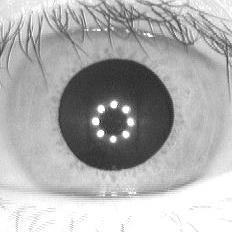
\includegraphics[width=44mm]{tfm-img21}}
\subfigure[S1001L01.jpg]{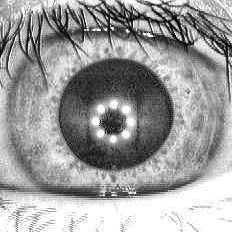
\includegraphics[width=44mm]{tfm-img22}}
\caption{Resultado de la aplicación del método de mejora de constraste CLAHE sobre una imagen de la base de datos CASIA-IrisV4-Internal. (a) Imagen original. (b) Resultado de aplicar el método CLAHE.} \label{fig:señales}
\end{figure}


\subsection{Extracción de las características basada en puntos de interés}

Dentro de los métodos de extracción de características podemos distinguir los que se centran en extraer características locales, normalmente basados en puntos de interés y que presentan un mayor robustez ante problemas de oclusión, objetos superpuestos, diferentes fuentes de ruido y perspectiva, y los métodos que se centran en extraer características globales, los cuales tienen cierta desventaja frente a los anteriores para el reconocimiento de iris en condiciones no ideales. Estos tipos de métodos basados en características globales parten de la desventaja de que no son capaces de diferenciar si un punto o característica pertenece al objeto o al fondo de la escena, requiriendo en estos casos aplicar operaciones adicionales como una segmentación más precisa del iris, lo que resulta bastante complejo en condiciones no ideales. Básicamente, los métodos de extracción de características locales basados en puntos de interés se conforman de un detector de puntos de interés y de un descriptor que describe la región alrededor de cada punto de interés. \\

Los puntos de interés son detectados en el espacio de escala. Para eso nos basamos en el supuesto de que los objetos tienen una propiedad innata en el mundo real por la cual estos sólo existen como entidades con sentido en un cierto rango de escalas. Mediante esta propiedad podemos comprobar como los objetos que son más relevantes en una imagen persisten, y como los menos significativos desaparecen. Para realizar este procedimiento lo que se hace es representar la imagen en múltiples escalas creando para ello un espacio de escala. Este espacio de escala se define como el resultado obtenido de la convolución de una escala variable Gaussiana \textit{G(x, y, z)} con la imagen de entrada \textit{I(x, y)}:\\

\[
L(x,y,\sigma) = G(x,y,\sigma) * I(x,y)
\]

En la siguiente figura se puede ver el efecto de emborronado que produce el cambio brusco de los valores variando el flitro en la función Gaussiana. \\ \\ \\

\begin{figure}[htbp]
\centering
\subfigure[]{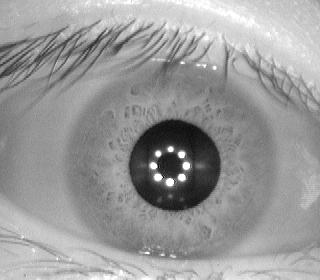
\includegraphics[width=50mm]{tfm-img24}}
\subfigure[]{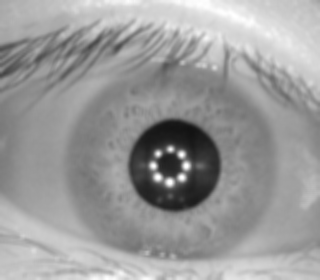
\includegraphics[width=50mm]{tfm-img25}}
\subfigure[]{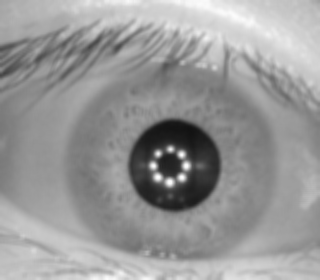
\includegraphics[width=50mm]{tfm-img26}}
\subfigure[]{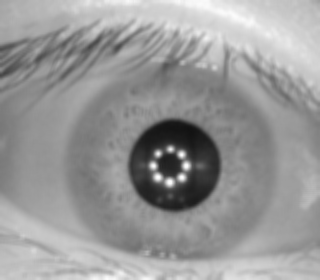
\includegraphics[width=50mm]{tfm-img27}}
\caption{Representación del espacio de escala sobre una imagen de la base de datos CASIA-IrisV4-Internal. (a) Imagen original. (b) $\sigma$ = 3. (c) $\sigma$ = 5. (d) $\sigma$ = 10.} \label{fig:señales}
\end{figure}

Los detectores de puntos de interes se basan en la búsqueda de características tales como esquinas, blobs y regiones dentro de la imagen, identificando en dichos lugares los puntos de interés que no varían en situaciones de transformaciones de escala, perspectiva y/o transformaciones afines. El propósito de los descriptores es el de extraer información discriminante alrededor de los puntos de interés. Estos se clasifican en 3 categorías: basados en distribuciones (SIFT, PCA-SIFT, GLOH, SURF), basados en técnicas de frecuencia espacial (Transformada de Fourier, Transformada de Gabor, Transformada de wavelet) y descriptores diferenciales (Filtros Steerable, Invariante diferencial). \\

El método de extracción de características que se propone en este Trabajo Fin de Master se encuadra dentro de los métodos de extracción de características locales, que como ya se ha visto se componen de un detector de puntos de interés y de un desciptor encargado de describir la región alrededor de cada punto. A diferencia de otros métodos de extracción de características existentes que emplean un único detector de puntos de interés, el método propuesto fusiona 3 detectores dentro del conjunto de los basados en la búsqueda de características en esquinas, blobs y regiones. Para mantener un equilibrio entre los seleccionados de estos tipos de detectores se ha realizado un estudio donde se pueda analizar los resultados que arrojarían utilizando varias combinaciones de estos detectores y descriptores para valorar cual sería la combinación óptima de los mismos \cite{Reference23} \cite{Reference24} \cite{Reference25}. Tras la evaluación investigada sobre las posibles combinaciones de detectores y descriptores, se ha llegado a la conclusión de que el resultado que proporciona un mayor interés en su investigación y que puede ser el más adecuado es el formado por la combinación de los detectores Harris-Laplace (detector de esquina), Hessian-Laplace (detector de blobs) y Fast-Hessian (detector de blobs). De entre todos los descriptores mencionados en el estado del arte, se ha seleccionado el descriptor SIFT como el encargado de caracterizar las regiones alrededor de cada punto de interés detectado debido que es el que mejor se integra con los detectores nombrados anteriormente. Además, este descriptor constituye la base de varios descriptores y como se ve en la siguiente figura representa un mayor grado de precisión frente a los demás descriptores. \\

\begin{figure}[htbp]
\centering
\subfigure{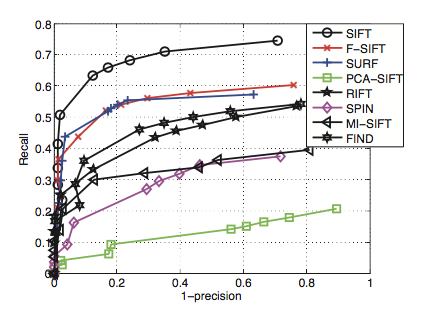
\includegraphics[width=110mm]{tfm-img51}}
\caption{Rendimiento de ocho descriptores diferentes con el detector DoG sobre 8 pares de imágenes que cubren transformaciones como escalado, rotación, cambios en el punto de vista, emborronado, cambios en el ratio de comprensión JPEG y cambios de iluminación.} \label{fig:señales}
\end{figure}


\subsubsection{Harris-Laplace}

El detector Harris \cite{Reference24} se basa principalmente en la matriz de segundo momento que es definida en la siguiente figura para un punto X.

\[
\mu (X, \sigma_{I}, \sigma_{D}) = \sigma_{D}^{2} g(\sigma_{I}) * \begin{bmatrix}
 L_{x}^{2}(X, \sigma_{D}) &  L_{x} L_{y}(X, \sigma_{D}) \\ 
  L_{x} L_{y}(X, \sigma_{D}) & L_{y}^{2}(X, \sigma_{D})
\end{bmatrix}
\]
\captionof{figure}{Ec. 1.1} 

donde $\sigma_{I}$ es la escala de integración, $\sigma_{D}$ es la escala de diferenciación y $ L_{g}$ es la derivada calculada en la dirección g (X o Y). Esta matriz describe principalmente la distribución del gradiente en un vecindario local de un punto X. Las derivadas locales son calculadas con núcleos (kernel) Gaussianos de un tamaño determinado por la escala local $\sigma_{D}$ (escala de diferenciación). Las derivadas son entonces promediadas entre los vecinos cercanos de los puntos por suavizado con una ventana Gaussiana de tamaño $\sigma_{I}$ (escala de integración). Los valores propios de esta matriz presenta dos cambios principales de señal en los vecinos cercanos de un punto. Basado en esta función, el detector Harris favorece a los pixeles que tienen grandes valores de curvatura en ambas direcciones principales. Por lo tanto, la función de selección es definida como muestra la siguiente figura. 

\[
Harris(X, \sigma_{I}, \sigma_{D}) = \left | \mu (X, \sigma_{I}, \sigma_{D}) \right | - \alpha*trace^{2}(\mu (X, \sigma_{I}, \sigma_{D}))
\]
\captionof{figure}{Ec. 1.2} 

donde $\alpha$ es una constante. En consecuencia, un punto de interés local es identificado donde un pixel alcanza un máximo local con respecto a las esquinas. \\

Para lograr la invarianza de escala, una escala apropiada debe ser elegida para cada punto de interés local detectado. Este proceso implica buscar extremos locales en el espacio de escala. En la matriz del segundo momento adaptada a la escala, el parámetro $\sigma_{I}$ determina la escala de la región local centrada en el punto X. Diferentes $\sigma_{I}$ dan como resultado diferentes máximos locales de función. Sin embargo, no todos los máximos locales generados por diferentes $\sigma_{I}$ son válidos.  Para simplificar el problema, $\sigma_{D}$ está relacionado con $\sigma_{I}$ por un ratio constante, por ejemplo, $\sigma_{D}$ = 0.8 · $\sigma_{I}$ . Como resultado, el problema de buscar parámetros apropiados para $\sigma_{D}$ y $\sigma_{I}$, se ha reducido la búsqueda de extremos locales en el espacio de escala. \\

Sin embargo, como indica T.Lindeberg \cite{Reference26}, la ecuación Ec. 1.2 rara vez alcanza los máximos en el espacio de escala. Por el contrario, si se mide la prominencia de la región con la función Laplaciana de Gauss en el espacio de escala, el extremo local en el espacio de escala puede ser definido con mas precisión.

\[
LoG(X, \sigma_{I}) = \sigma_{I}(L_{xx(x, \sigma_{I})} + L_{yy(x, \sigma_{I})})
\]
\captionof{figure}{Ec. 1.3} 

donde $L_{gg}$ indica la derivada de segundo orden en la dirección g. Como resultado, el detector Harris-Laplace en lugar de medir la prominencia para cada pixel como en la ecuación Ec. 1.2 solo, la Ec. 1.3 es también aplicada en cada pixel. Este proceso ha sido repetido en múltiples escalas. Los puntos de interés finales son localizados en el espacio X-Y donde la ecuación Ec. 1.2 alcanza el máximo local y la ecuación Ec. 1.3 alcanza el extremo local simultáneamente. \\


\subsubsection{Hessian-Laplace}

A diferencia del detector Harris, dada la matriz Hessian para un punto X.

\[
H(X, \sigma) = \begin{bmatrix}
 L_{xx}(X, \sigma) &  L_{xy}(X, \sigma)  \\ 
 L_{xy}(X, \sigma)  &  L_{yy}(X, \sigma))
\end{bmatrix}
\]
\captionof{figure}{Ec. 1.4} 

donde $\sigma$ es el parámetro de suavizado Gaussiano. La ecuación Ec. 1.6 define la prominencia de un punto X únicamente basado en el determinante de la matriz de Hessian. 

\[
H(X, \sigma) = \begin{bmatrix}
 L_{xx}(X, \sigma_{D}) &  L_{xy}(X, \sigma_{D})  \\ 
 L_{xy}(X, \sigma_{D})  &  L_{yy}(X, \sigma_{D}))
\end{bmatrix}
\]
\captionof{figure}{Ec. 1.5} 

De manera similiar a Harris-Laplace, se requiere seleccionar un parámetro $\sigma_{d}$ apropiado. Esto implica la construcción de un espacio de escala con la ecuación Ec. 1.5. Los puntos Hessian son por lo tanto definidos en la ecuación Ec. 1.5 que alcanza los extremos locales en el espacio de escala.. \\

Actualmente, para seleccionar apropiadamente $\sigma_{D}$ en el espacio de escala tenemos otra opción nombrada como la función Laplaciana de Gauss. Si los puntos detectados son requeridos para alcanzar el extremo local con la ecuación Ec. 1.3 en el espacio de escala, se define el nuevo detector Hessian-of-Laplacian. 

\[
H(X,\sigma) = det(H(X,\sigma))  *  \sigma^{4}
\]
\captionof{figure}{Ec. 1.6} 

\begin{table}[htbp]
\begin{center}
\end{center}
\end{table}

\begin{table}[htbp]
\begin{center}
\end{center}
\end{table}

\subsubsection{Fast-Hessian}
Fast Hessian es el detector de características SURF \cite{Reference27}. Su idea básica es calcular la ecuación Ec. 1.6 de una manera eficiente con la ayuda de imágenes integrales. Para permitir un cálculo rápido, la ecuación Ec. 1.6 ha sido aproximada a la ecuación Ec. 1.7.

\[
Det(H_{approx}) = D_{xx}D_{yy} - (0.9D_{xy})^{2}
\]
\captionof{figure}{Ec. 1.7} 

donde $D_{xx}$, $D_{yy}$ y $D_{xy}$ todos pueden ser calculados eficientemente usando filtros de caja. La detección es realizada en cuatro escalas y tres octavos (particiones de tamaño 8). Debido a la considerable pérdida en la aproximación, la localización de los puntos de interés en cualquier espacio de escala o espacio X-Y no puede ser precisa. Parecido al detector DoG, la expansión Taylor en la ecuación Ec. 1.7 es adoptada para aproximar la ubicación exacta de los extremos. En la implementación original de SURF, el detector había sido emparejado con el descriptor SURF por la preocupación existente en cuanto a la velocidad. \\


\subsubsection{SIFT}
Se ha demostrado que el descriptor SIFT tiene éxito en varias tareas tales como clasificación de objetos, generación de panorama e identificación de imagen ND. Dada una región normalizada de un punto de interés, SIFT genera un histograma 2-D en la región local. La región local se particiona en bloques. La figura 5.11 muestra el esquema de partición de SIFT. El gradiente de un píxel dentro de cada bloque de partición se ha cuantificado de acuerdo con su orientación. Normalmente, el número de contenedores de cuantificación es 8 \cite{Reference28}. Antes de la cuantificación, la región local es rotada a su orientación dominante. Esta operación permite que las características extraídas sean invariantes a las transformaciones de rotación. La orientación dominante se estima también en función de la cuantización de la orientación en el campo gradiente de la región local. Generalmente, la región usada para calcular la orientación dominante es una pequeña porción de la región local (por ejemplo, una parte concéntrica de la región local con longitud de radio la mitad). Para lograr un mejor rendimiento, el histograma se pondera adicionalmente en primer lugar	 por su longitud de gradiente, y en segundo lugar por una ventana Gaussiana centrada alrededor del punto de interés. \\

\begin{figure}[htbp]
\centering
\subfigure{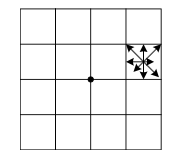
\includegraphics[width=60mm]{tfm-img52}}
\caption{SIFT} \label{fig:señales}
\end{figure}

%----------------------------------------------------------------------------------------